\chapter{Jednostránkové webové aplikace}
Jedním z aktuálních pojmů ve světě vývoje webových aplikací jsou takzvané Single Page Applications (SPA) neboli jednostránkové aplikace. Podle Osmani \cite{osmani_spa} lze SPA definovat jako webovou aplikaci, která se kompletně načte v prohlížeči, a poté se stará o navigaci a vykreslování HTML. Tím se SPA velmi liší od tradičního modelu, ve kterém jsou pohledy uživatelského rozhraní vždy vykreslovány serverem.

Jednostránkové aplikace bohatě využívají jazyk Javascript, který běží uvnitř webového prohlížeče uživatele. Využití webového prohlížeče pro manipulaci s HTML místo načítání pokaždé nové stránky, přispívá k větší uživatelské přívětivosti. Aplikace je velmi interaktivní, okamžitě reaguje na uživatelské vstupy a provádí aktualizace jen takových částí stránky, kde došlo ke změně. Jakákoliv další data, která jsou potřeba pro zobrazení obsahu uživateli, jsou dotahována dynamicky a na pozadí. 

Významně se také snižuje zátež webového serveru, ten u typické jednostránkové aplikace zpravidla vystupuje jen jako API, které dodává Javascriptové aplikaci data a provádí datové operace. Komunikace probíhá prostředníctví protokolu HTTP přes serverové REST rozhraní. Většinou se pro reprezentaci dat využívá formát JSON \cite{json}. Při programování SPA je tedy nutné striktně oddělovat backend a frontend. Frontend tvoří čistě Javascriptová aplikace běžíčí uvnitř webového prohlížeče, backend poskytuje data a provádí nad nimy změny. Jako serverovou část SPA lze použít některý ze známých webových frameworků, které poskytují podporu pro REST API. Knihovna schopná implementace REST rozhraní existuje pro téměř každý z běžně používaných programovacích jazyků \cite{spa_book} \cite{spa_web}. 

\pagebreak
Následující diagram dobře ilustruje rozdíly mezi klasickými a jednostránkovými webovými aplikacemi \cite{spa_diagram}.
\begin{figure}[h]
\begin{centering}
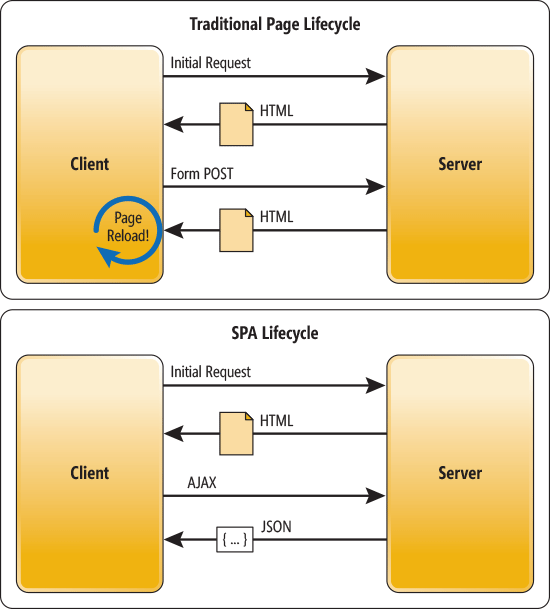
\includegraphics[scale=0.5]{obrazky/spa_vs_traditional}
\par\end{centering}
\caption{Diagram interakce klasické a jednostránkové webové aplikace \cite{spa_diagram}. \label{fig:spa_diagram}}
\end{figure}
\FloatBarrier

\section{Vznik myšlenky SPA}
Původní World Wide Web paradigma vzniklo pro jednoduché zobrazování statických HTML stránek uživateli pomocí webového prohlížeče. Pro stále se zvětšující rodinu webových aplikací je obvyklá představa webu coby sady provázaných hypertextových dokumentů nedostatečná.Ve chvíli, kdy se web začal měnit z \uv{knihovny dokumentů} na aplikační platformu, začala být evidentní potřeba změny tohoto modelu. Možnosti interakce původního HTTP se však omezují na vyžádání jiné webové stránky nebo odeslání formuláře na server k dalšímu zpracování. Takové požadavky uživatelů jsou vždy zpracovávany synchronně, v pořadí v jakém byly doručeny serveru. Každá uživatelská akce způsobí načtení celé nové HTML stránky. Tento princip slavil úspěch díky své jednoduchosti a vedl k masovému rozšíření webových prezentací po celém světě. Aplikace vždy dodržovaly pravidlo rozmístění funkcionality do více stránek, kdy každá stránka odpovídala určitému stavu, události nebo úkolu. Výhody tohoto postupu jsou zřejmé, například uložení jednotlivých stránek do záložek. Naopak nevýhodou může být přenos zbytečně velkých dat, která se posílají stále dokola. Jednoduchost HTTP protokolu, která pomohla rychlému rozšíření, se však později ukázala jako nevhodná pro tvorbu složitejších aplikací. Z jedné strany je jazyk HTML omezující pro webové vývojáře, kteří se musejí omezit na základní možnost úprav klasických formulářů prostřednictvím CSS stylů. Na straně druhé je matoucí pro uživatele, kteří jsou z klasických desktopových aplikací již zvykli na určité prvky a způsob jejich ovladání. Je také velmi neefektivní stahovat ze serveru vždy celou HTML stránku, potřebujeme-li změnit jen nějakou její malou část. V poslední době můžeme pozorovat snahu webových vývojářů příblížit svoje aplikace klasickým desktopovým aplikacím a poskytnout tak uživateli iluzi, že pracuje s běžnou aplikací. Jedná se o tak zvané \textit{jedno-stránkové webové aplikace (Single Page Applications – SPA)} \cite{spa} psané v Javascriptu. V takové aplikaci se veškeré nutné zdroje (kód, média a ostatní) nahrají najednou při načtení úvodní stránky a není již potřeba aplikaci znovu načítat. Veškerá komunikace se serverem se odehrává na pozadí, aniž by rušila dojem uživatele, že pracuje s klasickou desktopovou aplikací. Komunikace má vždy navic asynchronni charakter, který se pro vývoj v Javascriptu typický. Myšlenka tvorby jednostránkých webových aplikací vznikla postupným vývojem skupiny webových technologii, které dnes známe pod zkratkou AJAX. Nejdůležitější z nich, \textit{XMLHttpRequest}, je základní javascriptové rozhraní, které se používá pro asynchronní komunikaci mezi klientem a serverem \cite{xhr}. Komunikace probíhá na pozadí a nedochází při ní k faktickému přenačtení webové stránky. Do širšího povědomí se tyto technologie začaly dostávat kolem roku 2000. Od té doby následoval bouřlivý vývoj, který přinesl nové knihovny a utility, jež zjednodušovali vývoj AJAX aplikací. Nejznámější javascriptovou knihovnou, vzniklou v této době, je dodnes hojně použivané jQuery, které vzniklo v roce 2006. Tato knihovna přináší programátorovi dobře dokumentované rozhraní pro práci se strukturou HTML, asynchronní obsluhu událostí, komunikaci se serverem a podobně. jQuery dnes najdeme téměř na každém webu a jeho alespoň základní znalost je pro každého webového vývojáře takřka nezbytností. Nejednalo se však v té době o jednostránkové webové aplikace, knihovna jQuery sloužila pouze pro řízení některých částí stránky, které komunikovaly se serverem pomocí asynchronních událostí. Využití knihovny pro kompletní obsluhu webové stránky podle princpipu SPA je sice teoreticky možné, avšak v praxi nepraktické. Plné rozvinutí konceptu jednostránkové aplikace umožnil až nástup moderních javascriptových MVC frameworků jako AngularJS nebo ember.js, které vyšly kolem roku 2010. Tyto frameworky adoptovaly návrhový vzor Model – View – Controller (MVC) a výrazně tak usnadňují vývoj webových aplikací, neboť programátoři jsou na tento koncept zvyklí z jiných programovacích jazyků. Speciálně framework AngularJS byl navržen pro snadné použití u Java vývojářů \cite{angular}. Styl vývoje u těchto frameworků byl ve své době revoluční, kompletní logika webové aplikace – získávání a vykreslování dat, validace, nebo routování, se provádí uvnitř webových prohlížečů uživatelů. Proto typická jednostránková aplikace podstatně méně zatěžuje server. Server pouze poskytuje data a reaguje na událostí, tvoří tedy takzvané API. Zobrazování UI a veškeré interakce s uživatelem řídí Javascript \cite{spa_horyna} \cite{spa}. 

\section{Princip technologie}
Základním principem jednostránkových aplikací je spuštění celé webové aplikace při prvním načtení vstupního bodu aplikace, většinou se jedná o soubor index.html. S prvním přístupem jsou načteny všechny základní zdroje definované v hlavičce HTML dokumentu. Další zdroje jsou načítány až ve chvíli, kdy jsou skutečně potřeba, i tak je ale při prvním načtení nutné stáhnout a zpracovat velké množství dat. To je jedna z nevýhod jednostránkových webových aplikací. Stahování dalších dat nebo HTML šablon je plně v režii frameworku použitého pro vývoj. Komunikace probíhá pomocí technologie XHR, dle principu AJAX. Pomocí Javascriptu je ze serveru stažen další obsah (multimédia, HTML kód nebo text), ten je načten do paměti prohlížeče a dojde k plynulému překreslení nějaké části aplikace. Pomocí této techniky je možné měnit obsah uživateli \uv{pod rukama}, aniž bychom museli znovu načíst a vykreslit celý dokument, jak by bylo nutné u klasických webových aplikací. Stejným způsobem mohou být načítány i CSS soubory, nebo další javascriptové zdroje. U SPA běží celá aplikace uvnitř webového prohlížeče, kompletní aplikační logika je definována v Javascriptu a server je redukován na poskytovatele dat pomocí REST API. Hovoříme tedy o takzvaném \uv{tlustém klientu}. Možnost běhu celého aplikace pomocí javascriptového jádra webového prohlížeče umožnil jejich masivní vývoj posledních let a s ním spojený významný nárust jejich výkonnosti. Spuštění celé jednostránkové aplikace však značně zatěžuje procesor koncového zařízení, což je problém především u některých mobilních zařízení, které mají méně výkonné procesory. Následující diagram dobře ilustruje rozdělení rolí typické jednostránkové aplikace naprogramované v jazyce Javascript \cite{spa_book} \cite{spa_web}.

\begin{figure}[h]
\begin{centering}
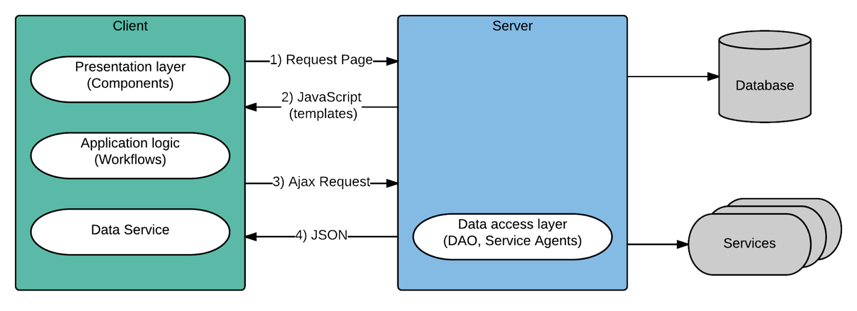
\includegraphics[scale=1]{obrazky/spa_architecture}
\par\end{centering}
\caption{Diagram typické architektury jednostránkové webové aplikace v javascriptu \cite{isomorhic_book} \label{fig:spa_architecture}}
\end{figure}

\section{Hlavní výhody}
Obecně se tato technologie hodí převážně pro weby, které počítají s velkou mírou interaktivity, mají tedy určitou logiku, kterou je nutné vyhodnocovat v prohlížeči. Prakticky se ale jako SPA dá naprogramovat jakákoliv webová aplikace, od statických prezentací až po velké informační systémy. Většina webových aplikací je dnes navrhována s ohledem na vysokou interaktivitu. Použití Javascriptu je proto u webových aplikací prakticky nutností. Veškerá datová komunikace probíhá pomocí AJAX, tento způsob se využívá také při \textit{lazy loadingu}, který obsah stránky vykreslí v několika krocích. U náročných stránek tím lze docílit rychlého zobrazení nejdůležitějšího obsahu, další méně důležité části lze načíst až později. Díky vysokému zapojení Javascriptu lze dnes většinu jednostránkových aplikací alespoň částečně používat také offline \cite{spa_book} \cite{spa_horyna}.

Následující kapitola shrnuje hlavní výhody jednostránkových webových aplikací, spolu se souvisejícími technologiemi, které je realizují.

\subsection{Větší míra interakce}
Standard HTML zná pouze několik základních vstupních prvků (tlačítka, textová pole, výběrové seznamy, zaškrtávací pole a další), pomocí kterých je realizována interakce uživatele s webovou aplikací. Větší míra zapojení Javascriptu umožňuje rozšířit tuto základní nabídku prvků, čímž je zlepšena intuitivnost a uživatelský prožitek (user experience) webové aplikace. Jako příklad lze uvést dialogová okna, funkci \textit{drag and drop}\footnote{Vyvolání nějaké akce přetáhnutím souboru do webového prohlížeče.}, nebo rozšířené formulářové prvky například pro výběr datumu či barvy. Také možnost využití přechodů nebo animací může zlepšit uživatelský prožitek \cite{spa_book} \cite{spa_horyna}.

Jednostránková javascriptová aplikace přestavuje takzvanou RIA (Rich Internet Application). Taková aplikace by se dala definovat jako webová aplikace, která se snaží nabídnout některé prvky klasických desktopových aplikací \cite{ria}. Mnoho z těchto nových prvků přináší standard HTML5, jenž je dnešními webovými prohlížeči velmi dobře podporován\cite{spa_book} \cite{spa_web}. HTML5 je nový standard značkovacího jazyka HTML vydaný v roce 2014, který přinesl \cite{janovsky_html5} \cite{html5_css3_book}:

\begin{itemize}
\item nové sémantické elementy: <article>, <aside>, <details>, <figcaption>, <figure>, <footer>, <header>, <main>, <mark>, <nav>, <section>, <summary>, <time>,
\item nové druhy vzhledu a chování formulářových polí <input>,
\item nový tag <datalist> pro výběr z více možností,
\item validaci formulářů a některé užitečné atributy formulářových polí, například placeholder,
\item tagy <video> a <audio>,
\item atribut download k odkazům vynucující stažení a určující jméno, souboru
\item lokální datová úložiště (asociativní pole, relační databáze), které je ale nutné obsluhovat Javascriptem,
\item javascriptem dostupná API na geolokaci, drag \& drop, web workers a SSE zjednodušení zápisů doctype a kódování stránky\
\item a mnohá další.
\end{itemize}

Lepší možnosti interakce přinesl do webových prohlížečů také nový standard stylovacího jazyka CSS. Verze CSS3 byla vydána konsorciem W3C (World Wide Web Consortium) v roce 2015 a dnes se dokončuje jeho implementace do webových prohlížečů \cite{css3} \cite{html5_css3_book}. Třetí verze přinesla především tyto novinky.

\begin{itemize}
\item \textbf{Media queries} – Umožňují aplikovat některé CSS deklarace jen po splnění určitých podmínek, většinou typu zobrazení a velikost rozlišení. Media queries je jedním ze tří pilířů responzivního webdesignu, spolu s fluidním layoutem a fluidními médii. Příklad použití: \textit{@media screen and (min-width : 500px) {h1 {color: blue}}} nastaví všem nadpisům modrou barvu, ale jen na rozlišení větší než 500px na šířku. 
\item \textbf{Nové selektory }např.: nth-child() , :nth-of-type(), checked().
\item \textbf{Vícesloupcový layout.}
\item \textit{Oblé rohy} – vlastnost border-radius dokáže definovat \uv{kulatost} rohů.
\item \textbf{Stínování} – vlastnost box-shadow přijímá čtyři parametry: horizontální posunutí stínu, vertikální posunutí stínu, okraj stínu a jeho barvu.
\item \textbf{Průhlednost} – pomocí vlastnosti opacity lze zprůhlednit jakýkoliv HTML objekt na stránce.
\item \textbf{CSS3 transformace} – vlastnost transform umožňuje změnu orientace, tvaru, perspektivy i velikosti objektů tedy různé přetáčení, překlápění nebo škálování.
\end{itemize}

Samotnou vysokou interaktivitu ale umožňuje především samotný Javascript, který realizuje veškeré DOM manipulace, na kterých je celá jednostránková aplikace založena \cite{spa_book} \cite{spa_web}. 

\subsection{Obnovování pouze určitých částí aplikace}
Jednou z velkých novinek moderních webových aplikací bylo odstranění nutnosti načítat a zobrazovat celou HTML stránku znovu při každé uživatelské akci. Neustálé čekání na načtení stránky může na uživatele působit rušivě a kazit jeho celkový dojem. Jednostránková webové aplikace v Javascriptu je kompletně načtena do prohlížeče při první návštěvě aplikace a veškerá další komunikace, přechody mezi stránkami nebo validace vstupních dat probíhají bez opakovaného načítání celé stránky. Díky tomuto chování bylo možné webové aplikace přiblížit k těm desktopovým, změny v aplikaci probíhají téměř v reálném čase a daná webová aplikace je tak uživatelsky přívětivější \cite{spa_book} \cite{spa_web}.

\subsection{Mohou běžet offline}
SPA lze implementovat i tak, aby bylo možné s ní omezeně pracovat i v době krátkodobé nedostupnosti internetového připojení. Změny provedené uživatelem v offline režimu se ukládají do některé z pamětí webového prohlížeče. Dobře se k tomu hodí nové HTML5 komponenty \textit{Application Cache} nebo \textit{Local Storage}. Ty umožňují ukládát stav aplikace do paměti prohlížeče nebo dokonce ukládat soubory na disk klientského počítače. V okamžiku navázání spojení dojde k odeslání lokálně uloženého stavu celé aplikace na webový server, tedy ke zpracování všech akcí, které uživatel provedl ve stavu offline \cite{spa_book} \cite{spa_web}.

\subsection{Lepší výkonnost}
Díky využití výpočetního výkonu webového prohlížeče pro obsluhu vykreslování a základních uživatelských akcí nejsou kladeny takové nároky na webový server. Obecně lze řici, že díky zapojení javascriptu pracuje jednostránková webová aplikace rychleji než klasická webová aplikace. Je to především proto, že se datová komunikace omezuje jen na nezbytně nutná data a veškeré obslužné operace probíhají na pozadí uvnitř webového prohlížeče, ale také díky přenesení zodpovědnosti za vykreslování HTML z webového serveru do prohlížeče. Díky protokolu Websocket lze komunikaci aplikace se serverem ještě zrychlit a optimalizovat \cite{spa_book} \cite{spa_web}.
\pagebreak

\section{Roztříštěnost koncových zařízení}
Moderní doba přinesla obrovskou škálu zařízení, pomocí nichž lze přistupovat na Internet. Internet se stále více posouvá z osobních počítačů do každodenního života. Jak je vidět na grafu \hyperref[fig:mobile_popularity]{3.3} používání internetu na mobilních zařízeních v posledních několika letech velmi stoupá \cite{mobile_popularity}. 

\begin{figure}[h]
\begin{centering}
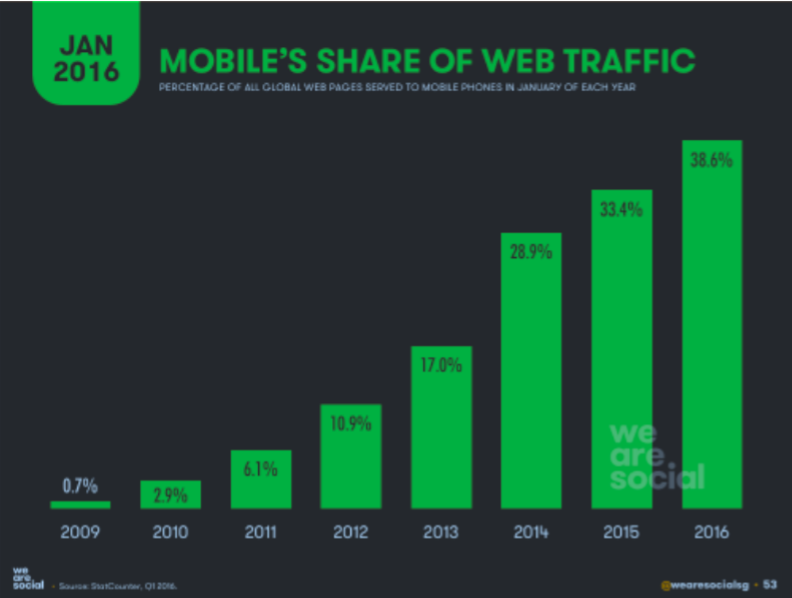
\includegraphics[scale=0.4]{obrazky/mobile_popularity}
\par\end{centering}
\caption{Vývoj zastoupení mobilních uživatelů na webu mezi lety 2009-2016 \cite{mobile_popularity}. \label{fig:mobile_popularity}}
\end{figure}
\FloatBarrier

Nástup mobilního internetu zvyšuje požadavky na návrh uživatelských rozhraní, která musí být schopná upravit zobrazení v závislosti na dostupném prostoru. Jak ukazuje obrázek \hyperref[fig:resolutions]{3.4} větší škála koncových zařízení přináší obrovské množství různých rozlišení. V praxi je nutné testovat web alespoň na klasickém počítači, mobilním telefonu a tabletu. Hovoříme tedy o takzvaném \uv{responzivním designu}. Jeho hlavní oblastí je adaptivní HTML layout. Je ale také nutné řešit rozdíly mezi javacriptovými jádry mobilních prohlížečů \cite{responsive_design}. Sjednocení běhových prostředí javacriptu se realizuje pomocí externích knihoven zvaných polyfillů, nejpoužívanější z nich je \textit{Modernizr}, který vedle doplnění nepodporovaných funkcí, poskytuje také rozhraní pro detekci novějších vlastností Javascriptu. Nedostupné funkce potom můžeme simulovat a tím zvýšíme kompatibilitu celé aplikace \cite{modernizr}.

\begin{figure}[h]
\begin{centering}
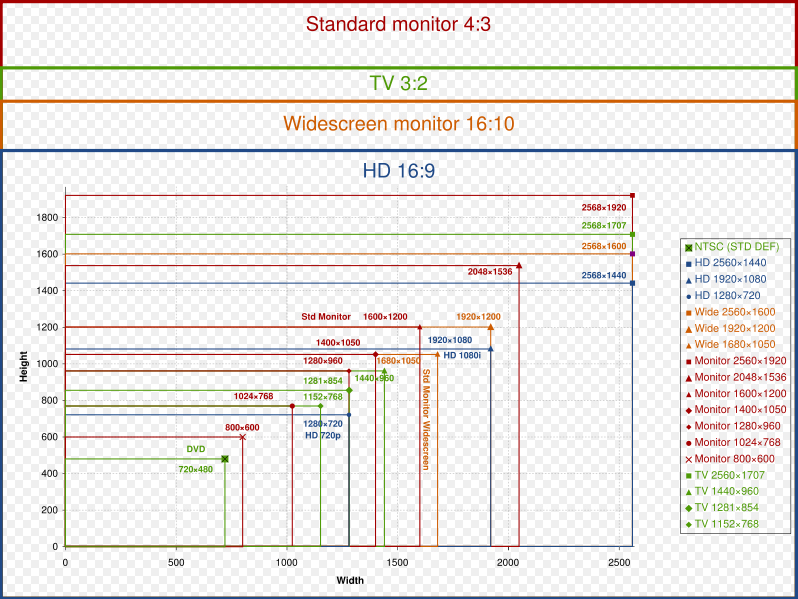
\includegraphics[scale=0.4]{obrazky/resolutions}
\par\end{centering}
\caption{Nejčastější rozlišení koncových zařízení na internetu \cite{mobile_popularity}. \label{fig:resolutions}}
\end{figure}
\FloatBarrier

\section{Vhodné knihovny}
Celý vývoj jednostránkových webových aplikace je hluboce založen na použití knihoven. Dobrý přehled poskytuje web TodoMVC \cite{todomvc}, kde je možné nalézt implementace jednoduchého úkolovníku ve většině javascriptových MVC frameworků. Mezi knihovny, které jsou pro SPA vhodné, patří například AngularJS, který představuje celý MVC framework, řeší tedy veškerou aplikační logiku uvnitř webového prohlížeče. Podobně orientované jsou také frameworky Backbone.js a Ember.js. Zatímco dnes popularní React se soustředí pouze na generování pohledu (view), tedy v našem případě cílového HTML kódu \cite{react}. Tento framework se nejčastěji používá jako zobrazovací vrstva u isomorfních aplikací a je také součástí ukázkové aplikace popsané v praktické části práce \cite{spa} \cite{spa_book}.

\vspace{0.3cm}
\noindent Některé často používané MVC frameworky:
\begin{itemize}
\item AngularJS,
\item BackboneJS,
\item EmberJS,
\item SpineJS,
\item SammyJS,
\item Knockout.js,
\item batman.js,
\item canjs.
\end{itemize}

\section{Nevýhody a časté problémy při vývoji}
Často zmiňovanou nevýhodou technologie jednostránkových aplikací je absolutní závislost na Javascriptu, který některá zařízení nemusí podporovat. Ačkoli podíl těchto zařízení stále klesá, problémem jsou především vyhledávací roboti. Mezi další nevýhody SPA patří \cite{spa_horyna}:

\begin{itemize}
\item časově, datově a výpočetně náročné první načtení webové aplikace, které je dané dobou načítání všech javascriptových zdrojů a dobou jejich zpracování jádrem webového prohlížeče,
\item celá aplikace se poskládána dynamicky, vyhledávací roboti (a uživatelé s vypnutým Javascriptem) jí mohou špatně zobrazit,
\item složitější implementace kvůli nutnosti správy aplikačního stavu,
\item problém s historií a tlačítkem zpět,
\item obrovské množství použitelných knihoven, problém vhodného výběru,
\item složitější příprava vývojového prostředí.
\end{itemize}

Jednou z problematických oblastí je také reakce jednostránkové aplikace na použití tlačítka zpět a obecně práce s URL a historií prohlížení. Tento problém se podařilo vyřešit až s rozšířením možností javascriptového API pro řízení historie a URL prohlížeč. Především velmi pomohlo doplnění možnosti ukládání stavu aplikace do historie prohlížeče. Jedná se o příkaz \textit{history.pushState()}. Pomocí něj lze zajistit stejné fungování historie jako u běžných serverových webových aplikací. Moderní javascriptové frameworky toto dnes řeší automaticky \cite{spa_book}.

Vyřešit problém špatné indexovatelnosti jednostránkových aplikací je mnohem složitější. Díky konceptu vykreslení celé aplikace pomocí Javascriptu, neexistuje jednoduché řešení, jak vyhledávacím robotům umožnit korektní zobrazení aplikace. Jedním z používaných řešení je spuštění takzvaného \uv{headless browseru}, tedy plnohodnotného webového prohlížeče bez grafického uživatelského rozhraní. Ten potom naslouchá na určené speciální URL, zpracuje celo jednostránkovou javascriptovou aplikaci a vrátí robotům kompletní HTML. Společnost Google doporučuje používat takzvanou \uv{hashbang notaci} 
( \#!aktualni-url) pro definici URL aplikace. Vyhledávací robot Googlu se potom pro adresu například 
\textit{www.example.com/\#!items/0/detail} pokusí získat její obsah na 
\textit{www.example.com/?\_escaped\_fragment=items/0/detail}, kde naslouchá zmiňovaný headless browser, který vrátí obsah pro vyhledávač \cite{google_crawler}. Celý proces ilustruje obrázek 
\hyperref[fig:prerender]{3.5}. Spuštění celého webového prohlížeče na serveru je ale velmi neefektivní a celé řešení vyžaduje složitou konfiguraci. Existují také externí služby, které vykreslování jednostránkových javascriptových aplikací pro vyhledávací roboty řeší, můžeme zmínit například Prerender.io \cite{prerender}. 

\begin{figure}[h]
\begin{centering}
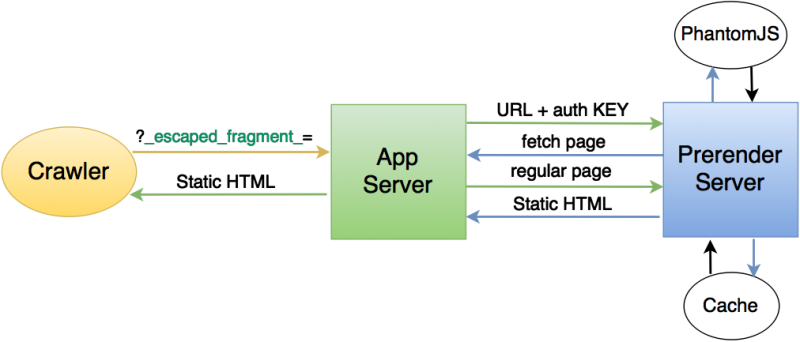
\includegraphics[scale=0.4]{obrazky/prerender}
\par\end{centering}
\caption{Diagram komunikace vyhledávacího robota s headless prohlížečem \cite{crawler_spa}. \label{fig:prerender}}
\end{figure}
\FloatBarrier

Mnohé z výše uvedených problémů řeší koncept isomorfních webových aplikací, který rozšířuje koncept SPA přenesením některých pravomocí zpět na webový server, který je také poháněn jazykem Javascript. Isomorfismus v kontextu webových aplikací znamená použití stejného jazyka pro server i webový prohlížeč \cite{universal_js}.